


%-------------------------------

\newpage

\section{Systematic Review and Modelography}{Revue Systématique et Modélographie}

\label{sec:modelography}

%-------------------------------


Tandis que les études menées précédemment proposaient de construire un horizon global de l'organisation des disciplines s'intéressant à notre question, nous proposons à présent une étude plus ciblée des caractéristiques de modèles existants. Nous proposons pour cela dans un premier temps une revue systématique, c'est à dire la construction d'un corpus plus précis répondant à certaines contraintes, suivie d'une meta-analyse, c'est à dire une tentative d'explication de certaines caractéristiques des modèles par des modèles statistiques.


%%%%%%%%%%%%%%%%%%%%
%\subsection[Systematic Review][Revue Systématique]{Systematic Review and Meta-analysis}{Revue systématique et Meta-analyse}
\subsection{Systematic Review and Meta-analysis}{Revue systématique et Meta-analyse}



Les revues systématiques classiques ont majoritairement lieu dans des domaines où une recherche très ciblée, même par titre d'article, fournira un certain nombre d'études étudiant quasiment la même question : typiquement en évaluation thérapeutique, où des études standardisées d'une même molécule varient uniquement par taille des effectifs et modalités statistiques (groupe de contrôle, placebo, niveau d'aveugle). Dans ce cas la construction du corpus est d'une part aisée par l'existence de bases spécialisées permettant des recherches très ciblées, et d'autre part par la possibilité de procéder à des analyses statistiques supplémentaires pour croiser les différentes études (par exemple meta-analyse par réseau, voir~\cite{rucker2012network}). Dans notre cas, l'exercice est bien plus aléatoire pour les raisons exposées dans les deux sections précédentes : les objets sont hybrides, les problématiques diverses, et les disciplines variées. Les différents points soulevés par la suite auront souvent autant de valeur thématique que de valeur méthodologique, suggérant des points cruciaux lors de la réalisation d'une telle revue systématique hybride.


Nous proposons une méthodologie hybride couplant les deux méthodologies développées précédemment avec une procédure plus classique de revue systématique. Nous souhaitons à la fois une représentativité de l'ensemble des disciplines que l'on a découvertes, mais aussi un bruit limité dans les références prises en compte pour la modélographie. Nous adoptons pour cela le protocole suivant :

% - 0.95% of edges with higher weight, with nodes in 80% quantile degree of their respective sem class.
% - take pairs (edges) and singles : 2582 kws
% - filter by hand : typically removed : Emissions, Education-cgnitive sci, teledetection, migration, social nws, lieux-pays, tourism-culture, social inequalities etc,  ; and too general : spillover e.g.  -> 115kws
% - request : can ask for 20 in that case
% - corpus : 2001 references
% - manual screening (title) 
%    * we already remove mobility studies (other scale) to limit final corpus
%    * pedestrian models
%    * traffic
%    * random stuffs
%    * design only (transport or lu independently) (≠ nw growth Tero)
%    * travel behavior : impact car ownersjip urb form, impact biofuel policies US, 
%    * ecology (habitat)
%    * technical transport
%    * pure eco (agllo eco) Anas urban spatial structure
%    * freight
%
%  -> N = 134 at this stage -> extend with corcit / hand
%  
% - manual screening citcore (N = 1843)
%    * rq : biaisé par titres pas explicites selon domaines (ex Courtat)
%  -> N' = 170
%
% - consolidation : N'' = 297
% 
% - full texts : 
%    * use of sci-hub necessary
%    * what do we mean by model ? (! contradiction with epistemo fwk ? clarifier) modèle de simulation / numérique.
%    * publishers ! : plus de springer, alors que que elsevier et tandf dans premiere section (corpus kws) -> biais request (et tous sur reasearch gate, like shady lit.)
%
% - final corpus : with Model = 145


\begin{enumerate}
\item Partant du corpus de citation isolé en~\ref{subsec:indirectbibliometrics}, nous isolons un nombre de mots-clés pertinents, en sélectionnant les 5\% de liens ayant le plus fort poids (seuil arbitraire), puis parmi les noeuds correspondants ceux ayant un degré supérieur au quantile à 0.8 de leur classe sémantique respective. Le premier filtrage permet de se concentrer sur le ``coeur'' des disciplines observées, et le second de ne pas biaiser par la taille sans perdre la structure globale, les classes étant relativement équilibrées. Un examen manuel permet de supprimer les mots-clés clairement non-pertinents (télédétection, tourisme, réseaux sociaux, \ldots), ce qui conduit à un corpus de $K=115$ mots-clés ($K$ est endogène ici).
\item Pour chaque mots-clé, nous effectuons automatiquement une requête au catalogue (scholar) en y ajoutant \texttt{model*}, d'un nombre fixé $n=20$ de références. L'ajout du terme est nécessaire pour obtenir des références pertinentes, après test sur des échantillons.
\item Le corpus potentiel composé des références obtenues, ainsi que des références composant le réseaux de citation, est revu manuellement (passage en revue des titres) pour assurer une pertinence au regard de l'état de l'art de~\ref{sec:modelingsa}, fournissant le corpus préliminaire de taille $N_p = 297$.
\item Ce corpus est alors inspecté pour les résumés et textes complets si nécessaire. On sélectionne les articles mettant en place une démarche de modélisation, hors modèles conceptuels. Les références sont classifiées et caractérisées selon des critères décrits ci-dessous. On obtient alors un corpus final de taille $N_f = 145$, sur lequel des analyses quantitatives sont possibles.
\end{enumerate}

La méthode est résumée en Fig.~\ref{fig:modelography:systematicreview}, avec les valeurs des paramètres et la taille des corpus successifs. Cet exercice permet tout d'abord un certain nombre de points méthodologiques, dont la connaissance pourra être un atout pour mener des revues systématiques hybrides similaires :

\begin{itemize}
\item Les biais de catalogue semblent inévitables. Nous reposons sur l'hypothèse que l'utilisation de Scholar permet un échantillonnage uniforme au regard des erreurs ou biais de catalogage. Le développement futur d'outils ouverts de catalogage et de cartographie, permettant un effort contributif pour une connaissance plus précise de domaines étendus et de leurs interfaces, sera un enjeu crucial de la fiabilité de ce genre de méthodes (voir~\ref{app:sec:cybergeo}).
\item La disponibilité des textes complets est particulièrement un problème pour une revue si large, vu la multiplicité des éditeurs. L'existence de moyens d'émancipation de la science ouverte comme Sci-hub\footnote{\url{http://sci-hub.cc/}} permet d'effectivement accéder à l'ensemble des textes. En écho au débat sur le bras de fer récent avec les éditeurs concernant l'exclusivité de la fouille de textes complets, il parait de plus en plus évident qu'une science ouverte réflexive est totalement antagoniste au modèle actuel de l'édition. Nous espérons également une évolution rapide des pratiques sur ce point.
\item Les revues, et en fait les éditeurs, semblent influencer différemment les référencements, augmentant potentiellement le biais de requête. La littérature grise ainsi que les pre-prints sont pris en compte différemment selon les champs.
\item Le passage en revue manuel des grand corpus permet de pas louper des ``poids lourds'' qui auraient pu être omis en amont~\cite{lissacksubliminal}. La question de la mesure dans laquelle on peut s'attendre d'être au courant de la manière la plus exhaustive des découvertes récentes liées au sujet étudié évolue très probablement vu l'augmentation de la quantité totale de littérature produite et la fragmentation des domaines pour certains toujours plus pointus~\cite{bastian2010seventy}. Rejoignant les points précédents, on peut supposer que des outils d'aide à l'analyse systématique permettront de garder cet objectif raisonnable.
\item Les résultats de la revue automatique sont sensiblement différents des domaines dessinés dans la revue classique : certaines associations conceptuelles, notamment l'inclusion des modèles de croissance de réseaux, ne sont pas naturelles et existent peu dans le paysage scientifique comme nous l'avons montré précédemment.
\end{itemize}


D'autre part, l'opération de construction du corpus permet déjà en elle-même de tirer des observations thématiques intéressantes en elles-mêmes :

\begin{itemize}
\item Les articles sélectionnés supposent une clarification de ce qui est entendu par ``modèle''. Nous donnons en~\ref{sec:knowledgeframework} une définition très large s'appliquant à l'ensemble des perspectives scientifiques. Notre selection ici ne retient pas les modèles conceptuels par exemple, notre critère de choix étant que le modèle doit inclure un aspect numérique ou de simulation.
\item Un certain nombre de références consistent en des revues, ce qui revient à un groupe de modèles ayant des caractéristiques similaires. On pourrait compliquer la méthode en retranscrivant chaque revue ou meta-analyse, ou en pondérant par le nombre d'article correspondant les enregistrements des caractéristiques correspondants. Nous faisons le choix d'ignorer ces revues, ce qui reste cohérent de manière thématique en restant dans l'hypothèse d'échantillonnage uniforme.
\item Une première clarification du cadre thématique est opérée, puisque nous ne sélectionnons pas les études liées uniquement au traffic et à la mobilité (ce choix étant aussi lié aux résultats obtenus en~\ref{sec:transportationequilibrium}), à l'urban design pur, au modèles de flux piétons, au fret, à l'écologie, aux aspects techniques du transport, pour donner quelques exemples, même si ces sujets peuvent dans une vue extrême être considérés comme liés aux interactions entre réseaux et territoires.
\item De la même façon, des domaines annexes comme le tourisme, les aspects sociaux de l'accès aux transports, l'anthropologie, n'ont pas été pris en compte.
\item On observe une forte fréquence des études liées au Trains à Grande Vitesse (HSR), rappelant la non-dissociabilité des aspects politiques de la planification et des directions de recherche en transports.%, surtout en France où les Corpsards des Ponts ou des Mines ont une main mise relative sur les deux aspects simultanément.
\end{itemize}


%%%%%%%%%%%%%%%
\begin{figure}[h!]
\frame{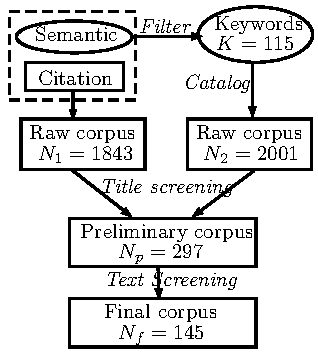
\includegraphics[width=\textwidth]{Figures/Modelography/systematicreview}}
\caption[Systematic Review][Méthodologie de la revue systématique]{\label{fig:modelography:systematicreview}}{\textbf{Méthodologie de la revue systématique.} Les rectangles désignent des corpus de références, les ellipses des corpus de mot-clés, et les pointillés les corpus initiaux. A chaque étape est donnée la taille du corpus.\label{fig:modelography:systematicreview}}
\end{figure}
%%%%%%%%%%%%%%%




%%%%%%%%%%%%%%%%%%%%
\subsection{Modelography}{Modélographie}

\comment[FL]{bien expliquer mais categories (?) dans figure 8 : curieux}

Nous passons à présent à une analyse mixte basée sur ce corpus, inspirée par les résultats des sections précédentes précédents notamment pour la classification. Elle a pour but d'extraire et de décomposer précisément les ontologies, échelles et processus, puis d'étudier des liens possibles entre ces caractéristiques des modèles et le contexte dans lequel ils ont été introduits. Il s'agit ainsi de la meta-analyse en quelque sorte, que nous désignerons ici par modélographie. Pour ne pas froisser les puristes, il ne s'agit en effet pas d'une meta-analyse à proprement parler car nous ne combinons pas des analyses proches pour extrapoler des résultats potentiels d'échantillons plus grand. Notre démarche est proche de celle de \noun{Cottineau} dans~\cite{2016arXiv160606162C} qui rassemble les références ayant étudié quantitativement la loi de Zipf pour les villes, puis lie les caractéristiques des études aux méthodes utilisées et hypothèses formulées.


La première partie consiste en l'extraction des caractéristiques des modèles. Automatiser ce travail constituerait un projet de recherche en lui-même, comme nous développons en discussion ci-dessous, mais nous sommes convaincus de la pertinence d'affiner de telles techniques (voir~\ref{ch:opening}) dans le cadre d'un développement de disciplines intégrées. Le temps étant autant l'ennemi que l'allié de la recherche, nous nous concentrons ici sur une extraction manuelle qui se voudra plus fine qu'une tentative peu convaincante de fouille de données. Nous extrayons des modèles les caractéristiques suivantes :

\begin{itemize}
\item Quelle est la force du couplage entre les ontologies territoriales et celles du réseau, autrement dit s'agit-il d'un modèle de co-évolution. Nous classerons pour cela en catégories suivant la représentation de la figure~\ref{fig:modelography:coevolution} : \texttt{\{territory ; network ; weak ; coevolution\}}, qui résulte de l'analyse de la littérature en~\ref{sec:modelingsa}.
\item Echelle de temps maximale. % et minimale (journalier, annuel, décade(s), siècle(s)) ; Multi-echelles temporelles (booléen)
\item Echelle d'espace maximale. %et minimale (local, ville, régional, système de ville) ; Multi-echelles spatiales (booléen)
\item Hypothèses d'équilibre.
\item Domaine ``a priori'', déterminé par l'origine des auteurs et domaine de la revue.
\item Méthodologie utilisée (modèles statistiques, système d'équations, multi-agent, automate cellulaire, recherche opérationnelle, simulation etc.).
\item Cas d'étude (ville, métropole, région ou pays) s'il y a lieu.
\end{itemize}

Nous collectons également de manière indicative, mais sans objectif d'objectivité ni d'exhaustivité, le ``sujet'' de l'étude (c'est à dire la question thématique dominante) ainsi que les ``processus'' inclus dans le modèle. Une extraction exacte des processus reste hypothétique, d'une part conditionnée à une définition rigoureuse et prenant en compte différents niveaux d'abstraction, de complexité, ou d'échelle, d'autre part dépendant de moyens techniques hors de portée de cette étude modeste. Nous commenterons ceux-ci de manière indicative sans les inclure dans les études systématiques.


%%%%%%%%%%%%%%%%%
\begin{figure}[h!]
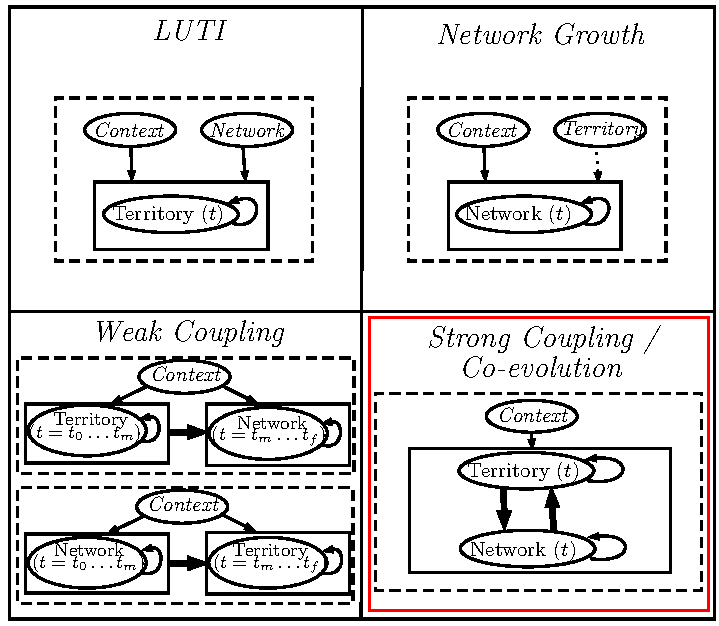
\includegraphics[width=\linewidth]{Figures/Modelography/coevolution}
\caption[Coupling types][Types de couplages]{Schematic representation of the distinction between different types of models coupling networks and territories \label{fig:modelography:coevolution}}{\textbf{Représentation schématique de la distinction entre différents types de modèles couplant territoires et réseaux.} Les ontologies sont représentés par des ovales, les sous-modèles par les boîtes pleines, les modèles par les boîtes pointillées, les couplages par les flèches. Nous surlignons en rouge l'approche qui sera l'objectif final de notre travail.\label{fig:modelography:coevolution}}
\end{figure}
%%%%%%%%%%%%%%%%%

Nous confondons également échelle, portée et dans un sens résolution pour ne pas rendre plus confus l'extraction. Même s'il serait pertinent de différencier lorsque un élément n'a pas lieu d'être pour un modèle (NA) de lorsque celui-ci est mal défini par son auteur, cette tâche apparaît sujette à subjectivité et nous fusionnons les deux modalités. Nous ajoutons aux caractéristiques ci-dessus les variables suivantes :

\begin{itemize}
\item Domaine de citation (le cas échéant, c'est à dire pour les références initialement présentes dans le réseau de citation, i.e. 55\% des références)
\item Domaine sémantique, défini par le domaine pour lequel le document a la plus grande probabilité
\item Indice d'interdisciplinarité
%\item Interdisciplinarité au second ordre (le cas échéant, pour les références consistant en les deux premiers niveaux du réseau de citation)
\end{itemize}

Les domaines sémantiques et la mesure d'interdisciplinarité ont été recalculés pour ce corpus par collecte des mots-clés, puis extraction selon la méthode décrite en~\ref{sec:quantepistemo}, avec $K_W=1000$, $\theta_w=15$ et $k_{max}=500$. On obtient des communautés plus ciblées et plutôt représentatives de la thématique et des méthodes : Transit-oriented development (\texttt{tod}), Hedonic models (\texttt{hedonic}), Planification des infrastructures (\texttt{infra planning}), High-speed rail (\texttt{hsr}) , Réseaux (\texttt{networks}), Réseaux complexes (\texttt{complex networks}), Bus rapid transit (\texttt{brt}).


Un ``bon choix'' de caractéristiques pour classer les modèles est un peu le problème du choix des \emph{features} en apprentissage statistique : si on est en supervisé, c'est à dire qu'on veut obtenir une bonne prédiction de classe fixée a priori (ou une bonne modularité de la classification obtenue par rapport à la classification fixée), on pourra sélectionner les caractéristiques optimisant cette prédiction. On discriminera ainsi les modèles que l'on connait et que l'on juge différents. Si l'on veut extraire une structure endogène sans a priori (classification non supervisée), la question est différente. Nous testerons pour cela en second temps une technique de regression qui permet d'éviter l'overfitting et faire de la selection de caractéristiques (forêts aléatoires).



\subsubsection{Processes and Case studies}{Processus et cas d'étude}

Concernant l'existence d'un cas d'étude et sa localisation, 26\% des études n'en présentent pas, correspondant à un modèle abstrait ou modèle jouet (la quasi totalité des études en physique tombant dans ce cas). Ensuite, elles sont réparties à travers le monde, avec toutefois une surreprésentation des Pays-bas avec 6.9\%. Les processus inclus sont trop variés (en fait autant que les ontologies des disciplines concernées) pour faire l'objet d'une typologie, mais on notera la domination de la notion d'accessibilité (65\% des études), puis des processus très variés allant de processus de marché immobilier pour les études hédoniques, aux relocalisations d'actifs et d'emplois pour les luti, ou aux investissements d'infrastructure de réseau. On observe des processus abstraits géométriques de croissance de réseau, correspondant aux travaux des physiciens. La maintenance du réseau apparait dans une étude, ainsi que l'histoire politique. Les processus abstraits d'agglomération et dispersion sont aussi le coeur de quelques études. Les interactions entre villes sont minoritaire, les approches de type système de villes étant noyées dans les études d'accessibilité. Les questions de gouvernance et de régulation ressortent aussi, plutôt dans le cas de planification d'infrastructure et de modèle d'évaluation de démarches TOD, mais sont aussi minoritaires. On retiendra que chaque domaine puis chaque étude introduit ses propres processus quasi-spécifiques à chaque cas.



\subsubsection{Corpus Characteristics}{Caractéristiques du corpus}

% DISCIPLINE
% biology computer science        economics      engineering      environment 
%       0.6896552        0.6896552       30.3448276        2.0689655        0.6896552 
%       geography          physics         planning   transportation 
%      19.3103448        8.2758621       20.0000000       17.9310345 
%
% SEMANTIC
%             brt complex networks          hedonic              hsr   infra planning 
%       0.6896552        0.6896552       11.0344828        2.7586207        5.5172414 
%        networks              tod 
%      20.6896552       27.5862069 

Les domaines ``a priori'' (i.e. jugés, ou plutôt préjugés sur la revue ou l'appartenance des auteurs), sont relativement équilibrés pour les disciplines majoritaires déjà identifiées : 17.9\% Transportation, 20.0\% Planning, 30.3\% Economics, 19.3\% Geography, 8.3\% physics, le reste minoritaire se répartissant entre environnement, informatique, ingénierie et biologie. Concernant les poids des domaines sémantiques significatifs, le TOD domine avec 27.6\% des documents, suivi par les réseaux (20.7\%), les modèles hédoniques (11.0\%), la planification des infrastructures (5.5\%) et le HSR (2.8\%). Les tables de contingences montrent que le Planning ne fait quasiment que du TOD, la physique uniquement des réseaux, la géographie se répartit équitablement entre réseaux et TOD (le second correspondant aux articles typés ``aménagement'', qui ont été classés en géographie car dans des revues de géographie) ainsi qu'une plus faible part en HSR, enfin l'économie est la plus variée entre hédonique, planning, réseaux et TOD. Cette interdisciplinarité n'apparait cependant que pour les classes extraites pour la probabilité majoritaire, puisque les indices d'interdisciplinarité moyens par discipline ont des valeurs équivalentes (de 0.62 à 0.65), hormis la physique significativement plus basse à 0.56 ce qui confirme son statut de ``nouveau venu'' ayant une profondeur thématique plus faible.


\subsubsection{Studied models}{Modèles étudiés}

Il est intéressant pour notre question de répondre à la question ``qui fait quoi ?'', c'est à dire quelles types de modèles sont mobilisés par les différentes disciplines. Nous donnons en Table~\ref{tab:modelography:what} la table de contingence du type de modèle en fonction des disciplines a priori, de la classe de citation et de la classe sémantique. On constate les approches fortement couplées, les plus proches de ce qu'on considère comme des modèles de co-évolution, sont majoritairement contenues dans le vocabulaire des réseaux, ce qui est confirmé par leur positionnement en terme de citation, mais que les disciplines concernées sont variées. La majorité des études s'intéresse au territoire uniquement, le déséquilibre le plus fort étant pour les études sémantiquement liées au TOD et à l'hédonique. La physique est encore limitée en s'intéressant exclusivement aux réseaux. 


%%%%%%%%%%%%%
\begin{table}
\caption[Model type][Type de modèles]{\textbf{Model types.}\label{tab:modelography:what}}{\textbf{Types de modèles étudiés selon les différentes classifications.} Tables de contingence de la variable discrete donnant le type de modèle (réseau, territoire ou couplage fort), pour la classification a priori, la classification sémantique et la classification de citation.\comment[FL]{a etoffer}\label{tab:modelography:what}}
\begin{tabular}{|m{2cm}|m{2cm}m{2cm}m{2cm}m{2cm}m{2cm}|}
\hline
Discipline  &  economics & geography & physics & planning & transportation\\\hline
network     &     5      &      3    &   12    &    1     &         4  \\
strong      &     4      &     3     &   0     &   0      &        2  \\
territory   &    35      &    22     &   0     &    28    &         20 \\\hline  
\end{tabular} 
\medskip
\begin{tabular}{|m{2cm}|m{2cm}m{2cm}m{2cm}m{2cm}m{2cm}|}
\hline
Semantic  &  hedonic & hsr & infra planning & networks & tod\\\hline
network   &       1  & 0   &          0     &  14      & 2 \\
strong    &       0  &  0  &            0   &     5    & 1  \\
territory &      15  &  4  &            8   &    11    &  37 \\ \hline
\end{tabular}
\begin{tabular}{|m{2cm}|m{2cm}m{2cm}m{2cm}m{2cm}m{2cm}m{2cm}|}
\hline
Citation  &  Accessibility & Geography & Infra Planning & LUTI & Networks & TOD \\\hline
network   &            0   &     0     &         0      &   0  &     24   &  0 \\
strong    &            0   &      0    &          0     &   2  &      5   &  0 \\
territory &           13   &      1    &          6     &  18  &      2   &  3 \\\hline
\end{tabular}
\end{table}
%%%%%%%%%%%%%



\subsubsection{Studied scales}{Echelles étudiées}

Pour répondre ensuite à la question du comment, on peut regarder les échelles de temps et d'espace typiques des modèles. La planification et les transports se concentrent à des petites échelles spatiales, métropolitain ou local, l'économie également avec une forte représentation du local via les études hédoniques, et une étendue un peu plus grande avec l'existence d'études au niveau régional et quelques une du pays (études de panel généralement). Encore une fois, la physique se retrouve limitée avec l'ensemble de ses contributions à une échelle fixe, métropolitaine (pas forcément claire ni bien spécifiée dans les articles d'ailleurs puisqu'il s'agit de modèles jouets dont les contours thématiques peuvent être très flous). La géographie est relativement bien équilibrée, de l'échelle métropolitaine à l'échelle continentale. Le schéma pour les échelles de temps est globalement similaire. Les méthodes utilisées sont fortement corrélées à la discipline : un test du $\chi^2$ donne une statistique de 169, très significatif avec $p=0.04$. De même, l'échelle d'espace l'est mais de manière moindre ($\chi^2 = 50, p = 0.08$).


\subsubsection{Classical Regressions}{Régressions classiques}

Nous étudions à présent l'influence de divers facteurs sur les caractéristiques des modèles par des régressions linéaires simples. Dans une démarche de multi-modélisation, nous proposons de tester l'ensemble des modèles possible pour expliquer chacune des variables à partir des autres. Le nombre d'observations pour lesquelles toutes les variables sont renseignées est très faible, il s'agit de prendre en compte le nombre d'observations utilisées pour ajuster chaque modèle. D'autre part, les performances du modèle peuvent être caractérisées par des objectifs complémentaires. Suivant~\cite{igel2005multi}, nous appliquons une optimisation multi-objectif, pour maximiser simultanément la variance expliquée (R$^2$ ajusté dans notre cas) et l'information capturée (Critère d'information d'Akaike corrigé AICc\footnote{L'AIC est une mesure du gain d'information entre deux modèles, et permet d'éviter l'ajustement abusif par un nombre trop grand de paramètres. L'AICc est une version prenant en compte la taille de l'échantillon, la mesure variant significativement pour les petits échantillons.}). Celle-ci est effectuée conditionnellement au fait d'avoir le nombre d'observations $N>50$ (seuil fixé au regard de la distribution de $N$ sur l'ensemble des modèles). La procédure d'optimisation est détaillée en Appendice~\ref{app:sec:quantepistemo} pour chaque variable. L'échelle de temps et l'interdisciplinarité présentent des compromis difficiles à départager, et nous ajustons les deux candidats. Les autres variables présentent des solutions dominantes et nous n'ajustons qu'un seul modèle.

\comment[JR]{clarifier modele / resultats - etoffer resultats}


Les résultats complets des régressions sont donnés en Tab.~\ref{tab:quantepistemo:regressions}. Les échelles temporelle et d'espace, ainsi que l'année, sont les variables les mieux expliquées au sens de la variance. L'échelle de temps est influencée très significativement par le type de modèle : territoire qui diminue celle-ci, ou couplage fort qui l'augmente. Le fait d'être en physique influe également significativement, et élargit la portée temporelle des modèles. Au contraire, les approches d'ingénierie (souvent design optimal d'un réseau de transport) correspondent à une courte durée.

Pour l'échelle d'espace, le fait d'être en géographie a une forte influence sur la portée spatiale des modèles : en effet, les études régionales et à l'échelle du système de villes sont bien l'apanage de la géographie. L'appartenance au domaine du transport augmente aussi faiblement la portée spatiale (voir significativité dans les regressions complètes en Appendice~\ref{app:sec:quantepistemo}). Aucune autre variable n'a une influence significative.
 
Le niveau d'interdisciplinarité est bien expliqué par l'année, qui l'influence de manière négative, ce qui confirme une augmentation des spécialisations scientifiques dans le temps. Les études économétriques des modèles hédoniques apparaissent très spécialisées. Enfin, l'année de publication est expliquée significativement et positivement par le type territoire et par le fait d'être en transports, ce qui signifierait une recrudescence récente d'un profil particulier d'études. Un examen du corpus suggère qu'il s'agit des études sur la grande vitesse, apparaissant comme une mode scientifique récente.




%%%%%%%%%%%%%%%%%
\begin{table}[!htbp]
\caption[][]{\textbf{Explanation of models characteristics.}}{\textbf{Explication des caractéristiques des modèles.} Résultats de l'estimation par moindres carrés (OLS) des modèles linéaires sélectionnés, pour chacune des variables à expliquer : échelle temporelle (TEMPSCALE), échelle spatiale (SPATSCALE), indice d'interdisciplinarité (INTERDISC), année de publication (YEAR).\label{tab:quantepistemo:regressions}}
\begin{tabular}{lcccccc} 
\footnotesize
\\[-1.8ex]\hline 
\hline \\[-1.8ex] 
 & \multicolumn{6}{c}{\textit{Variable expliquée:}} \\ 
\cline{2-7} 
 & \multicolumn{2}{c}{TEMPSCALE} & SPATSCALE & \multicolumn{2}{c}{INTERDISC} & YEAR \\ 
 & (1) & (2) & (3) & (4) & (5) & (6)\\ 
\hline \\[-1.8ex] 
 YEAR & 0.674 &  &  & $-$0.004$^{*}$ & $-$0.002$^{*}$ &  \\ 
  TYPEstrong &  & 100.271$^{***}$ &  &  & $-$0.026 &  \\ 
  TYPEterritory & $-$38.933$^{***}$ & $-$14.988 &  &  & 0.044 & 10.898$^{***}$ \\ 
  TEMPSCALE &  &  & $-$5.179 & $-$0.0003 &  & 0.035 \\ 
  FMETHODeq &  &  &  &  &  & $-$6.224 \\ 
  FMETHODmap &  &  &  &  &  & 4.747 \\ 
  FMETHODro &  &  &  &  &  & 6.128 \\ 
  FMETHODsem &  &  &  &  &  & 1.009 \\ 
  FMETHODsim &  &  &  &  &  & 5.153 \\ 
  FMETHODstat &  &  &  &  &  & $-$0.357 \\ 
  DISCIPLINEengineering & $-$52.107$^{*}$ & $-$9.609 & $-$154.461 & 0.144 &  & 13.486 \\ 
  DISCIPLINEenvironment & 17.110 & 17.886 & $-$5.878 & 0.092 &  & $-$3.668 \\ 
  DISCIPLINEgeography & 3.640 & 9.126 & 1,445.457$^{***}$ & 0.036 &  & 1.121 \\ 
  DISCIPLINEphysics & 46.879$^{*}$ & 77.897$^{***}$ & 292.559 & $-$0.103 &  & 3.392 \\ 
  DISCIPLINEplanning & 1.304 & 4.553 & $-$143.554 & $-$0.047 &  & $-$2.850 \\ 
  DISCIPLINEtransportation & $-$14.718 & 8.753 & 568.329 & 0.062 &  & 5.503$^{*}$ \\ 
  INTERDISC & 2.357 &  &  &  &  & $-$12.876 \\ 
  SEMCOMcomplex networks &  &  &  &  & $-$0.217 &  \\ 
  SEMCOMhedonic &  &  &  & $-$0.179 & $-$0.184$^{*}$ & $-$5.769 \\ 
  SEMCOMhsr &  &  &  & $-$0.100 & $-$0.122 & 6.135 \\ 
  SEMCOMinfra planning &  &  &  & $-$0.032 & $-$0.096 & $-$4.123 \\ 
  SEMCOMnetworks &  &  &  & $-$0.038 & $-$0.107 & 4.711 \\ 
  SEMCOMtod &  &  &  & $-$0.105 & $-$0.152 & $-$1.653 \\ 
  Constant & $-$1,305.126 & 22.103$^{*}$ & 235.357 & 8.962$^{**}$ & 5.531$^{**}$ & 2,004.945$^{***}$ \\ 
 \hline \\[-1.8ex] 
Observations & 64 & 94 & 94 & 64 & 98 & 64 \\ 
R$^{2}$ & 0.385 & 0.393 & 0.100 & 0.314 & 0.155 & 0.510 \\ 
R$^{2}$ ajusté & 0.282 & 0.336 & 0.027 & 0.136 & 0.068 & 0.281 \\ 
%Residual Std. Error & 26.984 (df = 54) & 31.747 (df = 85) & 1,995.272 (df = 86) & 0.109 (df = 50) & 0.107 (df = 88) & 6.617 (df = 43) \\ 
%F Statistic & 3.755$^{***}$ (df = 9; 54) & 6.871$^{***}$ (df = 8; 85) & 1.369 (df = 7; 86) & 1.761$^{*}$ (df = 13; 50) & 1.789$^{*}$ (df = 9; 88) & 2.234$^{**}$ (df = 20; 43) \\ 
\hline 
\hline \\[-1.8ex] 
\textit{Note:}  & \multicolumn{6}{l}{$^{*}$p$<$0.1; $^{**}$p$<$0.05; $^{***}$p$<$0.01} \\ 
\end{tabular}
\end{table} 
%%%%%%%%%%%%%%%%%




\subsubsection{Random Forest Regressions}{Régressions par Forêts Aléatoires}

Nous concluons cette étude par des régressions et classification par Forêts Aléatoires, qui sont une méthode très flexible permettant de dégager une structure d'un jeu de données~\cite{liaw2002classification}. Pour compléter les analyses précédentes, nous proposons de l'utiliser pour déterminer les importances relatives des variables pour différents aspects. Nous utilisons à chaque fois des forêts de taille 100000, une taille de noeud de 1 et un nombre de variable échantillonnée en $\sqrt{p}$ pour la classification et $p/3$ pour la régression lorsque $p$ est le nombre total de variables. Pour classifier le type de modèle, nous comparons les effets de la discipline, de la classe sémantique et de la classe de citation. Cette dernière est la plus importante avec une mesure relative de 45\%, tandis que la discipline compte pour 31\% et le sémantique pour 23\%. Ainsi, le cloisonnement disciplinaire se retrouve, tandis que le sémantique et donc en partie les ontologies, est le plus ouvert. Cela nous encourage dans notre démarche de sortir de ce cloisonnement. Lorsqu'on applique une regression de forêt sur l'interdisciplinarité, toujours avec ces trois variables, on constate qu'elles expliquent 7.6\% de la variance totale, ce qui est relativement faible, témoignant d'une disparité de sémantique sur l'ensemble du corpus indépendamment des différentes classifications. Dans ce cas, la variable la plus importante est la discipline (39\%) suivie par le sémantique (31\%) et la citation (29\%), ce qui confirme que le journal visé conditionne fortement le comportement de langage employé. Cela nous alerte sur le danger de perte de richesse sémantique lorsqu'on s'adresse à un public particulier. Ainsi, nous avons pu dégager certaines structures et régularités des modèles nous concernant, qui seront riches d'enseignements lors de la construction de nos modèles.


\comment[JR]{que tire-t-on de tout ça ?}


%%%%%%%%%%%%%%%%%%%%
\subsection{Discussion}{Discussion}


\subsubsection{Further Developments}{Développements}

\bpar{
Further work may consist in the production of an automatic synthesis of this meta-analysis, from a modular modeling point of view, combined with a refined purpose and scale classification. Modular modeling consists in the integration of heterogeneous processes and implementation of processes in order to extract the set of mechanisms giving the best fit to empirical data~\cite{cottineau2015incremental}. We can thus classify models described here according to their building bricks in terms of processes implemented and thus identify possible coupling potentialities.
}{
Un développement possible pourrait consister en la mise en place d'une approche automatique à cette meta-analyse, du point de vue de la modélisation modulaire, combiné avec une classification du but et de l'échelle. La modélisation modulaire consiste en l'intégration de processus hétérogènes et d'implémentation de ces processus dans le but d'extraire les mécanismes donnant la meilleure proximité à des faits stylisés empiriques ou à des données~\cite{cottineau2015incremental}. L'idée serait de pouvoir extraire automatiquement la structure modulaire des modèles existants, à partir des textes complets comme proposé en~\ref{sec:quantepistemo}, afin de classifier ces briques de manière endogène et identifier des couplages potentiels pour des nouveaux modèles.
}



\subsubsection{Lessons for Modeling}{Leçons pour la modélisation}


Nous pouvons résumer les points principaux issus de cette méta-analyse qui joueront sur notre attitude et nos choix de modélisation. Tout d'abord, la présence interdisciplinaire des approches effectuant un couplage fort confirme notre besoin de faire des ponts et de coupler les approches, et confirme également rétrospectivement les conclusions de~\ref{sec:quantepistemo} sur les conséquences du cloisonnement des disciplines en terme de modèles formulés. Ensuite, l'importance du vocabulaire des réseaux dans une grande partie des modèles nous poussera à confirmer cet ancrage. La spécificité des approches TOD et d'accessibilité, assez proches des modèles LUTI, seront secondaires pour nous. La portée restreinte des travaux issus de la physique, confirmée par la majorité des critères étudiés, nous pousse à nous méfier de ces travaux et de l'absence de sens thématique aux modèles. La richesse des échelles temporelles et spatiale couvertes par les modèles géographiques et économiques nous confirme l'importance de varier celles-ci dans nos modèles, idéalement de parvenir à des modèles multi-échelles. Enfin, les importances relatives des variables de classification sur le type de modèle vont également dans le sens de ponts interdisciplinaires pour croiser les ontologies.







\stars



